\section{第四章 组合逻辑电路 作业}
% 这是子文件，可直接用 \input{文件名} 引入主文档

\subsection{题4.3：组合逻辑电路功能分析}
\subsubsection{题目}
分析图 P4.3 电路的逻辑功能，写出 $Y_1$、$Y_2$ 的逻辑函数式，列出真值表，指出电路完成什么逻辑功能。

\begin{center}
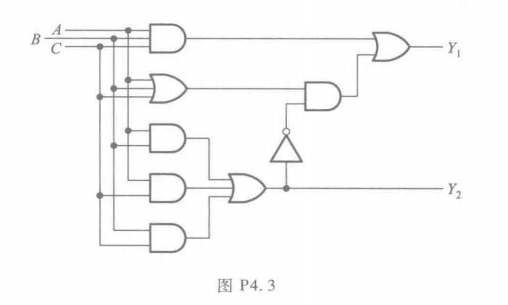
\includegraphics[width=0.6\textwidth]{4.3.png}
\end{center}
题4.3 逻辑电路图

\subsubsection{解答}
\begin{enumerate}
    \item \textbf{写出逻辑表达式}
    \begin{itemize}
        \item 由电路图逐级推导输出逻辑函数：
        \[
        Y_2 = AB + BC + AC
        \]
        \[
        Y_1 = ABC + (A+B+C) \cdot \overline{Y_2}
        \]
        \item 代入 $Y_2$ 并化简：
        \[
        \begin{aligned}
        Y_1 &= ABC + (A+B+C)\overline{AB+BC+AC} \\
        &= A\overline{B}\overline{C} + \overline{A}B\overline{C} + \overline{A}\overline{B}C + ABC \\
        &= A \oplus B \oplus C
        \end{aligned}
        \]
        \item 最终最简逻辑式：
        \[
        \boxed{Y_1 = A \oplus B \oplus C,\quad Y_2 = AB + BC + AC}
        \]
    \end{itemize}

    \item \textbf{列出真值表}
    \begin{center}
    \begin{tabular}{ccc|cc}
        \toprule
        $A$ & $B$ & $C$ & $Y_1$ & $Y_2$ \\
        \midrule
        0 & 0 & 0 & 0 & 0 \\
        0 & 0 & 1 & 1 & 0 \\
        0 & 1 & 0 & 1 & 0 \\
        0 & 1 & 1 & 0 & 1 \\
        1 & 0 & 0 & 1 & 0 \\
        1 & 0 & 1 & 0 & 1 \\
        1 & 1 & 0 & 0 & 1 \\
        1 & 1 & 1 & 1 & 1 \\
        \bottomrule
    \end{tabular}
    \end{center}

    \item \textbf{逻辑功能分析}
    \begin{itemize}
        \item $Y_1 = A \oplus B \oplus C$：三变量异或，为 \textbf{全加器和位}，输入 1 的个数为奇数时输出为 1。
        \item $Y_2 = AB+BC+AC$：多数表决逻辑，为 \textbf{全加器进位位}，输入 1 的个数大于等于 2 时输出为 1。
        \item 整个电路为标准 \textbf{1 位全加器}，$Y_1$ 为和位 $S$，$Y_2$ 为进位输出 $C_O$。
    \end{itemize}
\end{enumerate}

\subsection{题4.5：用与非门设计四变量多数表决电路}
\subsubsection{题目}
用与非门设计四变量的多数表决电路。当输入变量 $A$、$B$、$C$、$D$ 有 3 个或 3 个以上为 1 时输出为 1，输入为其他状态时输出为 0。

\subsubsection{解答}
\begin{enumerate}
    \item \textbf{列出真值表}
    \begin{center}
    \begin{tabular}{cccc|c}
        \toprule
        $A$ & $B$ & $C$ & $D$ & $Y$ \\
        \midrule
        0 & 0 & 0 & 0 & 0 \\
        0 & 0 & 0 & 1 & 0 \\
        0 & 0 & 1 & 0 & 0 \\
        0 & 0 & 1 & 1 & 0 \\
        0 & 1 & 0 & 0 & 0 \\
        0 & 1 & 0 & 1 & 0 \\
        0 & 1 & 1 & 0 & 0 \\
        0 & 1 & 1 & 1 & 1 \\
        1 & 0 & 0 & 0 & 0 \\
        1 & 0 & 0 & 1 & 0 \\
        1 & 0 & 1 & 0 & 0 \\
        1 & 0 & 1 & 1 & 1 \\
        1 & 1 & 0 & 0 & 0 \\
        1 & 1 & 0 & 1 & 1 \\
        1 & 1 & 1 & 0 & 1 \\
        1 & 1 & 1 & 1 & 1 \\
        \bottomrule
    \end{tabular}
    \end{center}

    \item \textbf{写出逻辑表达式并化简为与非-与非形式}
    \begin{itemize}
        \item 从真值表写出标准最小项和式：
        \[
        Y = \sum m(7,11,13,14,15)
        \]
        \item 卡诺图化简得到最简与或式：
        \[
        Y = ABC + ABD + ACD + BCD
        \]
        \item 两次取反转换为与非-与非形式：
        \[
        Y = \overline{\overline{ABC + ABD + ACD + BCD}}
        = \overline{\overline{ABC} \cdot \overline{ABD} \cdot \overline{ACD} \cdot \overline{BCD}}
        \]
    \end{itemize}

    \item \textbf{逻辑功能分析}
    \begin{itemize}
        \item 输入 $A,B,C,D$ 中有 3 个或 4 个为 1 时输出 1，否则输出 0，实现 \textbf{四变量多数表决器}。
        \item 表达式已化为与非-与非形式，可直接用两级与非门实现。
    \end{itemize}
\end{enumerate}

\subsection{题4.6：水箱水泵控制逻辑电路设计}
\subsubsection{题目}
有一水箱由大、小两台水泵 $M_L$ 和 $M_S$ 供水，如图 P4.6 所示。水箱中设置了 3 个水位检测元件 A、B、C。水面低于检测元件时，检测元件给出高电平；水面高于检测元件时，检测元件给出低电平。现要求：
\begin{itemize}
    \item 当水位超过 C 点时水泵停止工作；
    \item 水位低于 C 点而高于 B 点时 $M_S$ 单独工作；
    \item 水位低于 B 点而高于 A 点时 $M_L$ 单独工作；
    \item 水位低于 A 点时 $M_L$ 和 $M_S$ 同时工作。
\end{itemize}
试用门电路设计一个控制两台水泵的逻辑电路，要求电路尽量简单。

\begin{center}
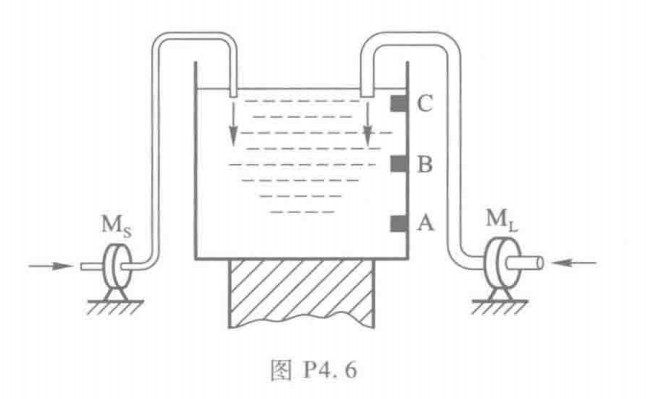
\includegraphics[width=0.6\textwidth]{4.6.png}
\end{center}
题4.6 水箱水泵控制示意图

\subsubsection{解答}
\begin{enumerate}
    \item \textbf{定义逻辑变量}
    \begin{itemize}
        \item 输入：$A,B,C$，高电平（1）表示水位低于该点，低电平（0）表示高于该点。
        \item 输出：$M_L$（大泵）、$M_S$（小泵），1=工作，0=停止。
    \end{itemize}

    \item \textbf{列出真值表（含所有输入状态与无关项）}
    \begin{center}
    \begin{tabular}{ccc|cc|c}
        \toprule
        $A$ & $B$ & $C$ & $M_L$ & $M_S$ & 工作状态 \\
        \midrule
        0 & 0 & 0 & 0 & 0 & 超过C点，全停 \\
        0 & 0 & 1 & 0 & 1 & B~C之间，仅$M_S$工作 \\
        0 & 1 & 0 & \multicolumn{2}{c}{×} & 不可能状态（无关项） \\
        0 & 1 & 1 & 1 & 0 & A~B之间，仅$M_L$工作 \\
        1 & 0 & 0 & \multicolumn{2}{c}{×} & 不可能状态（无关项） \\
        1 & 0 & 1 & \multicolumn{2}{c}{×} & 不可能状态（无关项） \\
        1 & 1 & 0 & \multicolumn{2}{c}{×} & 不可能状态（无关项） \\
        1 & 1 & 1 & 1 & 1 & 低于A点，双泵工作 \\
        \bottomrule
    \end{tabular}
    \end{center}

    \item \textbf{写出逻辑表达式并化简}
    \begin{itemize}
        \item 对 $M_L$ 化简：
        \[
        M_L = B
        \]
        \item 对 $M_S$ 化简：
        \[
        M_S = \overline{B}C
        \]
        \item 验证：
        \begin{itemize}
            \item 水位超过C：$A=B=C=0 \Rightarrow M_L=0,\ M_S=0$（正确）
            \item 水位B~C间：$A=0,B=0,C=1 \Rightarrow M_L=0,\ M_S=1$（正确）
            \item 水位A~B间：$A=0,B=1,C=1 \Rightarrow M_L=1,\ M_S=0$（正确）
            \item 水位低于A：$A=1,B=1,C=1 \Rightarrow M_L=1,\ M_S=1$（正确）
        \end{itemize}
    \end{itemize}

    \item \textbf{逻辑电路图说明}
    \begin{itemize}
        \item $M_L = B$：直接由输入 $B$ 控制，无需门电路。
        \item $M_S = \overline{B}C$：使用一个**非门**（对B取反）和一个**与门**（连接$\overline{B}$和C）实现。
        \item 整体电路最简，完全满足题目所有控制要求。
    \end{itemize}
\end{enumerate}

\subsection{题4.12：用74HC138实现多输出逻辑函数}
\subsubsection{题目}
试画出用3线-8线译码器74HC138（见图4.4.7）和门电路产生如下多输出逻辑函数的逻辑图。
\[
\begin{cases}
Y_1 = AC \\
Y_2 = \overline{A}\overline{B}C + A\overline{B}\overline{C} + BC \\
Y_3 = \overline{B}\overline{C} + AB\overline{C}
\end{cases}
\]

\begin{center}
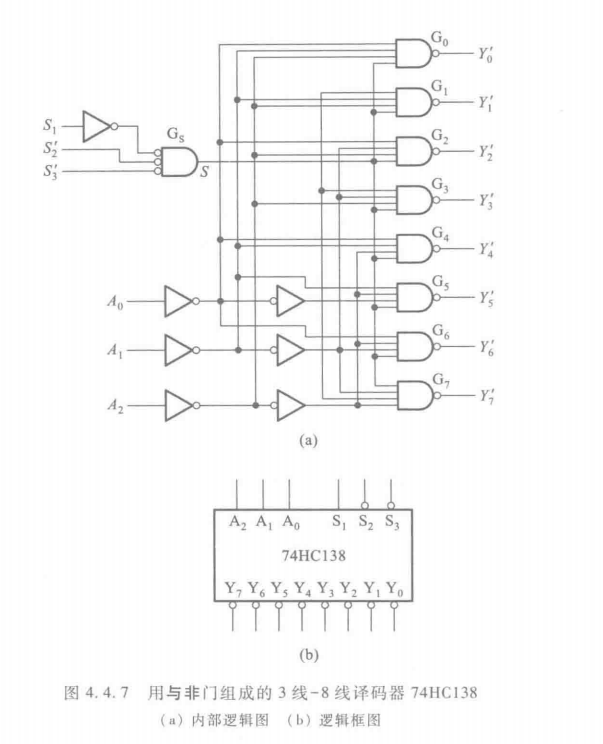
\includegraphics[width=0.6\textwidth]{4.4.7.png}
\end{center}
图4.4.7 74HC138逻辑符号

\subsubsection{解答}
\begin{enumerate}
    \item \textbf{将函数转换为标准与或式（最小项和形式）}
    \begin{itemize}
        \item 令地址高位到低位：$A_2=A,\ A_1=B,\ A_0=C$。
        \item $Y_1 = AC = A(B+\overline{B})C = ABC + A\overline{B}C = \sum m(5,7)$
        \item $Y_2 = \overline{A}\overline{B}C + A\overline{B}\overline{C} + BC
        = \overline{A}\overline{B}C + A\overline{B}\overline{C} + \overline{A}BC + ABC
        = \sum m(1,3,4,7)$
        \item $Y_3 = \overline{B}\overline{C} + AB\overline{C}
        = \overline{A}\overline{B}\overline{C} + A\overline{B}\overline{C} + AB\overline{C}
        = \sum m(0,4,6)$
    \end{itemize}

    \item \textbf{利用译码器输出实现逻辑函数}
    \begin{itemize}
        \item 74HC138 输出低电平有效：$\overline{Y_i} = \overline{m_i}$。
        \item 或运算转为与非形式：$\displaystyle Y=\sum m_i = \overline{\prod \overline{m_i}}$。
        \[
        Y_1 = \sum m(5,7) = \overline{\overline{Y_5} \cdot \overline{Y_7}}
        \]
        \[
        Y_2 = \sum m(1,3,4,7) = \overline{\overline{Y_1} \cdot \overline{Y_3} \cdot \overline{Y_4} \cdot \overline{Y_7}}
        \]
        \[
        Y_3 = \sum m(0,4,6) = \overline{\overline{Y_0} \cdot \overline{Y_4} \cdot \overline{Y_6}}
        \]
    \end{itemize}

    \item \textbf{逻辑电路连接说明}
    \begin{itemize}
        \item 输入 $A,B,C$ 分别接 74HC138 地址端 $A_2,A_1,A_0$；
        \item 使能端 $S_1$ 接高电平，$\overline{S_2},\overline{S_3}$ 接低电平，译码器正常工作；
        \item 外接与非门对对应译码器输出做与非运算，即可实现 $Y_1,Y_2,Y_3$。
    \end{itemize}
\end{enumerate}

\subsection{题4.16：用74HC151数据选择器实现逻辑函数}
\subsubsection{题目}
分析图 P4.16 电路，写出输出 $Z$ 的逻辑函数式。74HC151 为 8 选 1 数据选择器，它的逻辑图见图 4.5.5，输出的逻辑函数式见式(4.5.6)。

\begin{center}
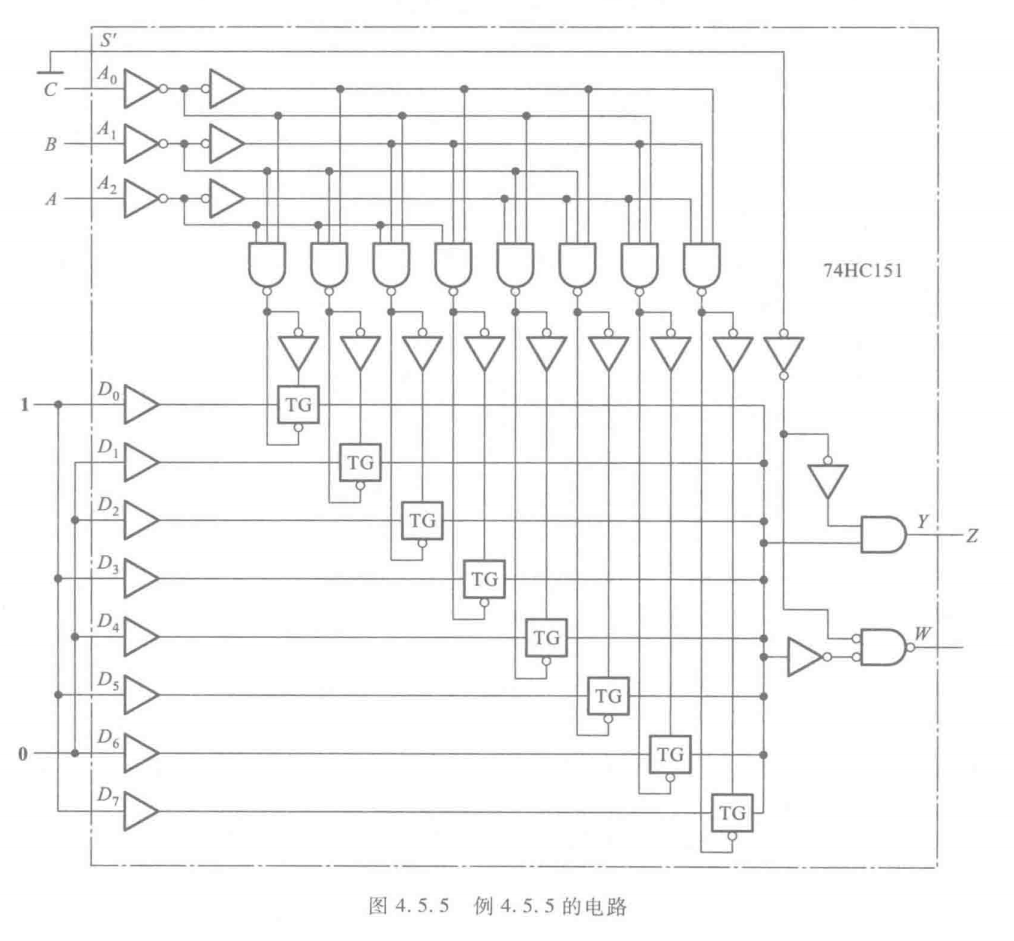
\includegraphics[width=0.6\textwidth]{4.5.5.png}
\end{center}
图4.5.5 74HC151逻辑符号

\begin{center}
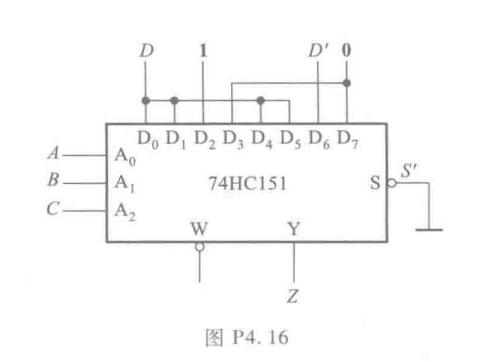
\includegraphics[width=0.6\textwidth]{4.16.png}
\end{center}
图P4.16 电路示意图

\subsubsection{解答}
\begin{enumerate}
    \item \textbf{分析数据选择器输入与输出关系}
    \begin{itemize}
        \item 74HC151 输出表达式：
        \[
        Y = \sum_{i=0}^{7} m_i D_i
        \]
        $m_i$ 为地址 $A_2A_1A_0$ 最小项，$D_i$ 为数据输入。
        \item 地址：$A_2=C,\ A_1=B,\ A_0=A$。
        \item 数据输入：
        \[
        D_0=D,\ D_1=D,\ D_2=1,\ D_3=1,\ D_4=\overline{D},\ D_5=\overline{D},\ D_6=0,\ D_7=0
        \]
        \item 使能端低电平有效，芯片工作，$Z=Y$。
    \end{itemize}

    \item \textbf{写出并化简输出逻辑函数}
    \begin{itemize}
        \item 代入展开：
        \[
        \begin{aligned}
        Z &= \overline{C}\overline{B}\overline{A}D + \overline{C}\overline{B}A D
        + \overline{C}B\overline{A} \cdot 1 + \overline{C}B A \cdot 1 \\
        &\quad + C\overline{B}\overline{A}\overline{D} + C\overline{B}A \overline{D}
        \end{aligned}
        \]
        \item 合并化简：
        \[
        Z = \overline{C}\overline{B}D + \overline{C}B + C\overline{B}\overline{D}
        \]
    \end{itemize}

    \item \textbf{逻辑功能分析}
    \begin{itemize}
        \item 电路实现四变量逻辑函数 $Z(A,B,C,D) = \overline{C}\overline{B}D + \overline{C}B + C\overline{B}\overline{D}$，由 8 选 1 数据选择器直接实现。
    \end{itemize}
\end{enumerate}

\subsection{题4.18：用4选1数据选择器产生逻辑函数}
\subsubsection{题目}
试用4选1数据选择器产生逻辑函数：
\[
Y = A\overline{B}\overline{C} + \overline{A}\overline{C} + BC
\]

\subsubsection{解答}
\begin{enumerate}
    \item \textbf{将函数转换为标准与或式}
    \begin{itemize}
        \item 展开为最小项：
        \[
        \begin{aligned}
        Y &= A\overline{B}\overline{C} + \overline{A}(B+\overline{B})\overline{C} + (A+\overline{A})BC \\
        &= A\overline{B}\overline{C} + \overline{A}B\overline{C} + \overline{A}\overline{B}\overline{C}
        + ABC + \overline{A}BC \\
        &= \sum m(0,1,2,3,6,7)
        \end{aligned}
        \]
    \end{itemize}

    \item \textbf{选择地址变量并确定数据输入}
    \begin{itemize}
        \item 取地址 $A_1=A,\ A_0=B$，4选1输出：
        \[
        Y = \overline{A}\overline{B}D_0 + \overline{A}B D_1 + A\overline{B}D_2 + AB D_3
        \]
        \item 按变量分组：
        \[
        Y = \overline{A}\overline{B}\,\overline{C} + \overline{A}B \cdot 1 + A\overline{B}\,\overline{C} + AB \cdot 1
        \]
        \item 对应数据输入：
        \[
        D_0 = \overline{C},\quad D_1 = 1,\quad D_2 = \overline{C},\quad D_3 = 1
        \]
    \end{itemize}

    \item \textbf{电路实现说明}
    \begin{itemize}
        \item 地址 $A,B$ 接选择器地址端 $A_1,A_0$；
        \item $D_0,D_2$ 接 $\overline{C}$，$D_1,D_3$ 接高电平；
        \item 使能端接地，即可实现给定逻辑函数。
    \end{itemize}
\end{enumerate}

\subsection{题4.23：用74HC151实现双功能控制电路}
\subsubsection{题目}
用8选1数据选择器74HC151设计一个组合逻辑电路。该电路有3个输入逻辑变量 $A,B,C$ 和1个工作状态控制变量 $M$。
当 $M=0$ 时实现“意见一致”功能（$A,B,C$ 状态一致时输出为1）；
当 $M=1$ 时实现“多数表决”功能。

\begin{center}
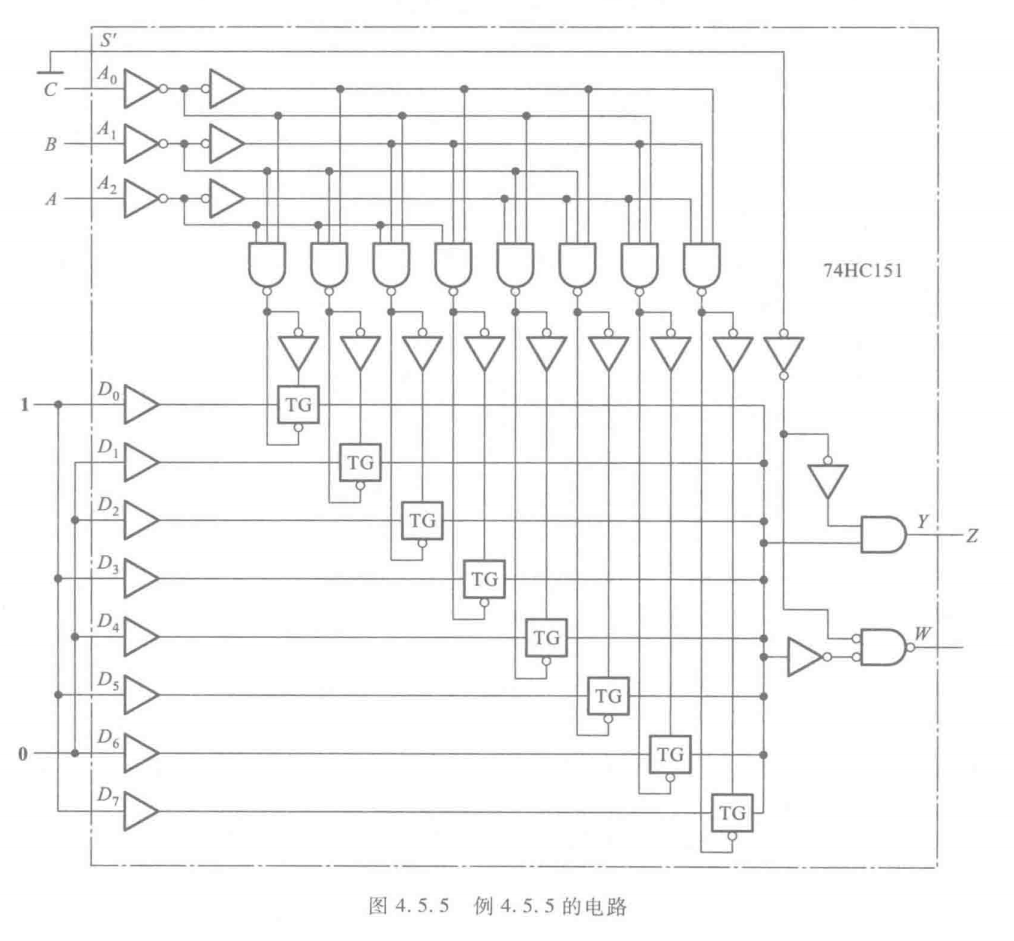
\includegraphics[width=0.6\textwidth]{4.5.5.png}
\end{center}
图4.5.5 74HC151逻辑符号

\subsubsection{解答}
\begin{enumerate}
    \item \textbf{列出输出逻辑函数的真值表}
    \begin{center}
    \begin{tabular}{cccc|c}
        \toprule
        $M$ & $A$ & $B$ & $C$ & $Y$ \\
        \midrule
        0 & 0 & 0 & 0 & 1 \\
        0 & 0 & 0 & 1 & 0 \\
        0 & 0 & 1 & 0 & 0 \\
        0 & 0 & 1 & 1 & 0 \\
        0 & 1 & 0 & 0 & 0 \\
        0 & 1 & 0 & 1 & 0 \\
        0 & 1 & 1 & 0 & 0 \\
        0 & 1 & 1 & 1 & 1 \\
        1 & 0 & 0 & 0 & 0 \\
        1 & 0 & 0 & 1 & 0 \\
        1 & 0 & 1 & 0 & 0 \\
        1 & 0 & 1 & 1 & 1 \\
        1 & 1 & 0 & 0 & 0 \\
        1 & 1 & 0 & 1 & 1 \\
        1 & 1 & 1 & 0 & 1 \\
        1 & 1 & 1 & 1 & 1 \\
        \bottomrule
    \end{tabular}
    \end{center}

    \item \textbf{选择地址变量并确定数据输入}
    \begin{itemize}
        \item 地址端 $A_2=A,\ A_1=B,\ A_0=C$；
        \[
        Y = \sum_{i=0}^{7} m_i D_i
        \]
        \item 由真值表得：
        \[
        \begin{aligned}
        D_0 &= 1,\quad D_1 = 0,\quad D_2 = 0,\quad D_3 = M \\
        D_4 &= 0,\quad D_5 = M,\quad D_6 = M,\quad D_7 = 1
        \end{aligned}
        \]
    \end{itemize}

    \item \textbf{电路实现说明}
    \begin{itemize}
        \item $A,B,C$ 接 74HC151 地址输入端 $A_2,A_1,A_0$；
        \item 数据端按 $D_0\sim D_7$ 分别接 $1,0,0,M,0,M,M,1$；
        \item 使能端接地，芯片工作，由 $M$ 切换两种逻辑功能。
    \end{itemize}
\end{enumerate}